\chapter{Results}
\label{ch:Results}
We show the results of the different experiments and discuss their implications.

\section{Hyperparameter Search}
We list the selected learning rate and regularization parameter for the five folds of each experiment (Tab~\ref{tab:HSResults}). Although hyperparameters were selected independently in each fold, they converge to similar values for the same experiment.
\begin{table}[h]
	\centering
	\setlength\tabcolsep{3.5pt}
	\begin{tabular}{l*{10}{c}}
		\hline
		 & \multicolumn{2}{c}{\textbf{Fold 1}} & \multicolumn{2}{c}{\textbf{Fold 2}} &\multicolumn{2}{c}{\textbf{Fold 3}} &\multicolumn{2}{c}{\textbf{Fold 4}} &\multicolumn{2}{c}{\textbf{Fold 5}}\\
		& \textbf{$\alpha$} & \textbf{$\lambda$} & \textbf{$\alpha$} & \textbf{$\lambda$} & \textbf{$\alpha$} & \textbf{$\lambda$} & \textbf{$\alpha$} & \textbf{$\lambda$} & \textbf{$\alpha$} & \textbf{$\lambda$}\\
		\hline 
		Exp. 1.1	&\sn{2}{-4}	&\sn{3}{-2}	&\sn{2}{-4}	&\sn{4}{-2}	&\sn{9}{-5}	&\sn{5}{-3}	&\sn{6}{-4}	&\sn{8}{-3}	&\sn{6}{-4}	&\sn{1}{-2}\\
		Exp. 1.2	&\sn{4}{-4}	&\sn{9}{-2}	&\sn{4}{-4}	&\sn{5}{-2}	&\sn{4}{-4}	&\sn{7}{-3}	&\sn{3}{-4}	&\sn{5}{-3}	&\sn{6}{-4}	&\sn{3}{-2}\\
		Exp. 1.3	&\sn{4}{-4}	&\sn{3}{-2}	&\sn{2}{-4}	&\sn{4}{-2}	&\sn{7}{-5}	&\sn{6}{-3}	&\sn{4}{-4}	&\sn{8}{-2}	&\sn{8}{-4}	&\sn{3}{-2}\\
		Exp. 2		&\sn{1}{-5}	&\sn{4}{-4}	&\sn{5}{-5}	&\sn{4}{-3}	&\sn{5}{-5}	&\sn{1}{-3}	&\sn{1}{-5}	&\sn{2}{-4}	&\sn{5}{-5}	&\sn{2}{-4}\\
		Exp. 3		&\sn{1}{-4}	&\sn{4}{-4}	&\sn{7}{-5}	&\sn{5}{-4}	&\sn{1}{-4}	&\sn{7}{-4}	&\sn{7}{-5}	&\sn{2}{-4}	&\sn{8}{-5}	&\sn{9}{-5}\\
		\hline
	\end{tabular}
	\caption[Selected hyperparameters]{Selected learning rate and regularization parameter configurations.}
	\label{tab:HSResults}
\end{table}

\section{Experiments}
Models perform similarly while commiting few errors (Fig.~\ref{fig:FROCResults}): different models perform better at different false positive per image marks but overall diferences are small. Furthermore, performance varies significantly among different folds of the same experiment making inferences harder.
\begin{figure}[h]
	\centering
		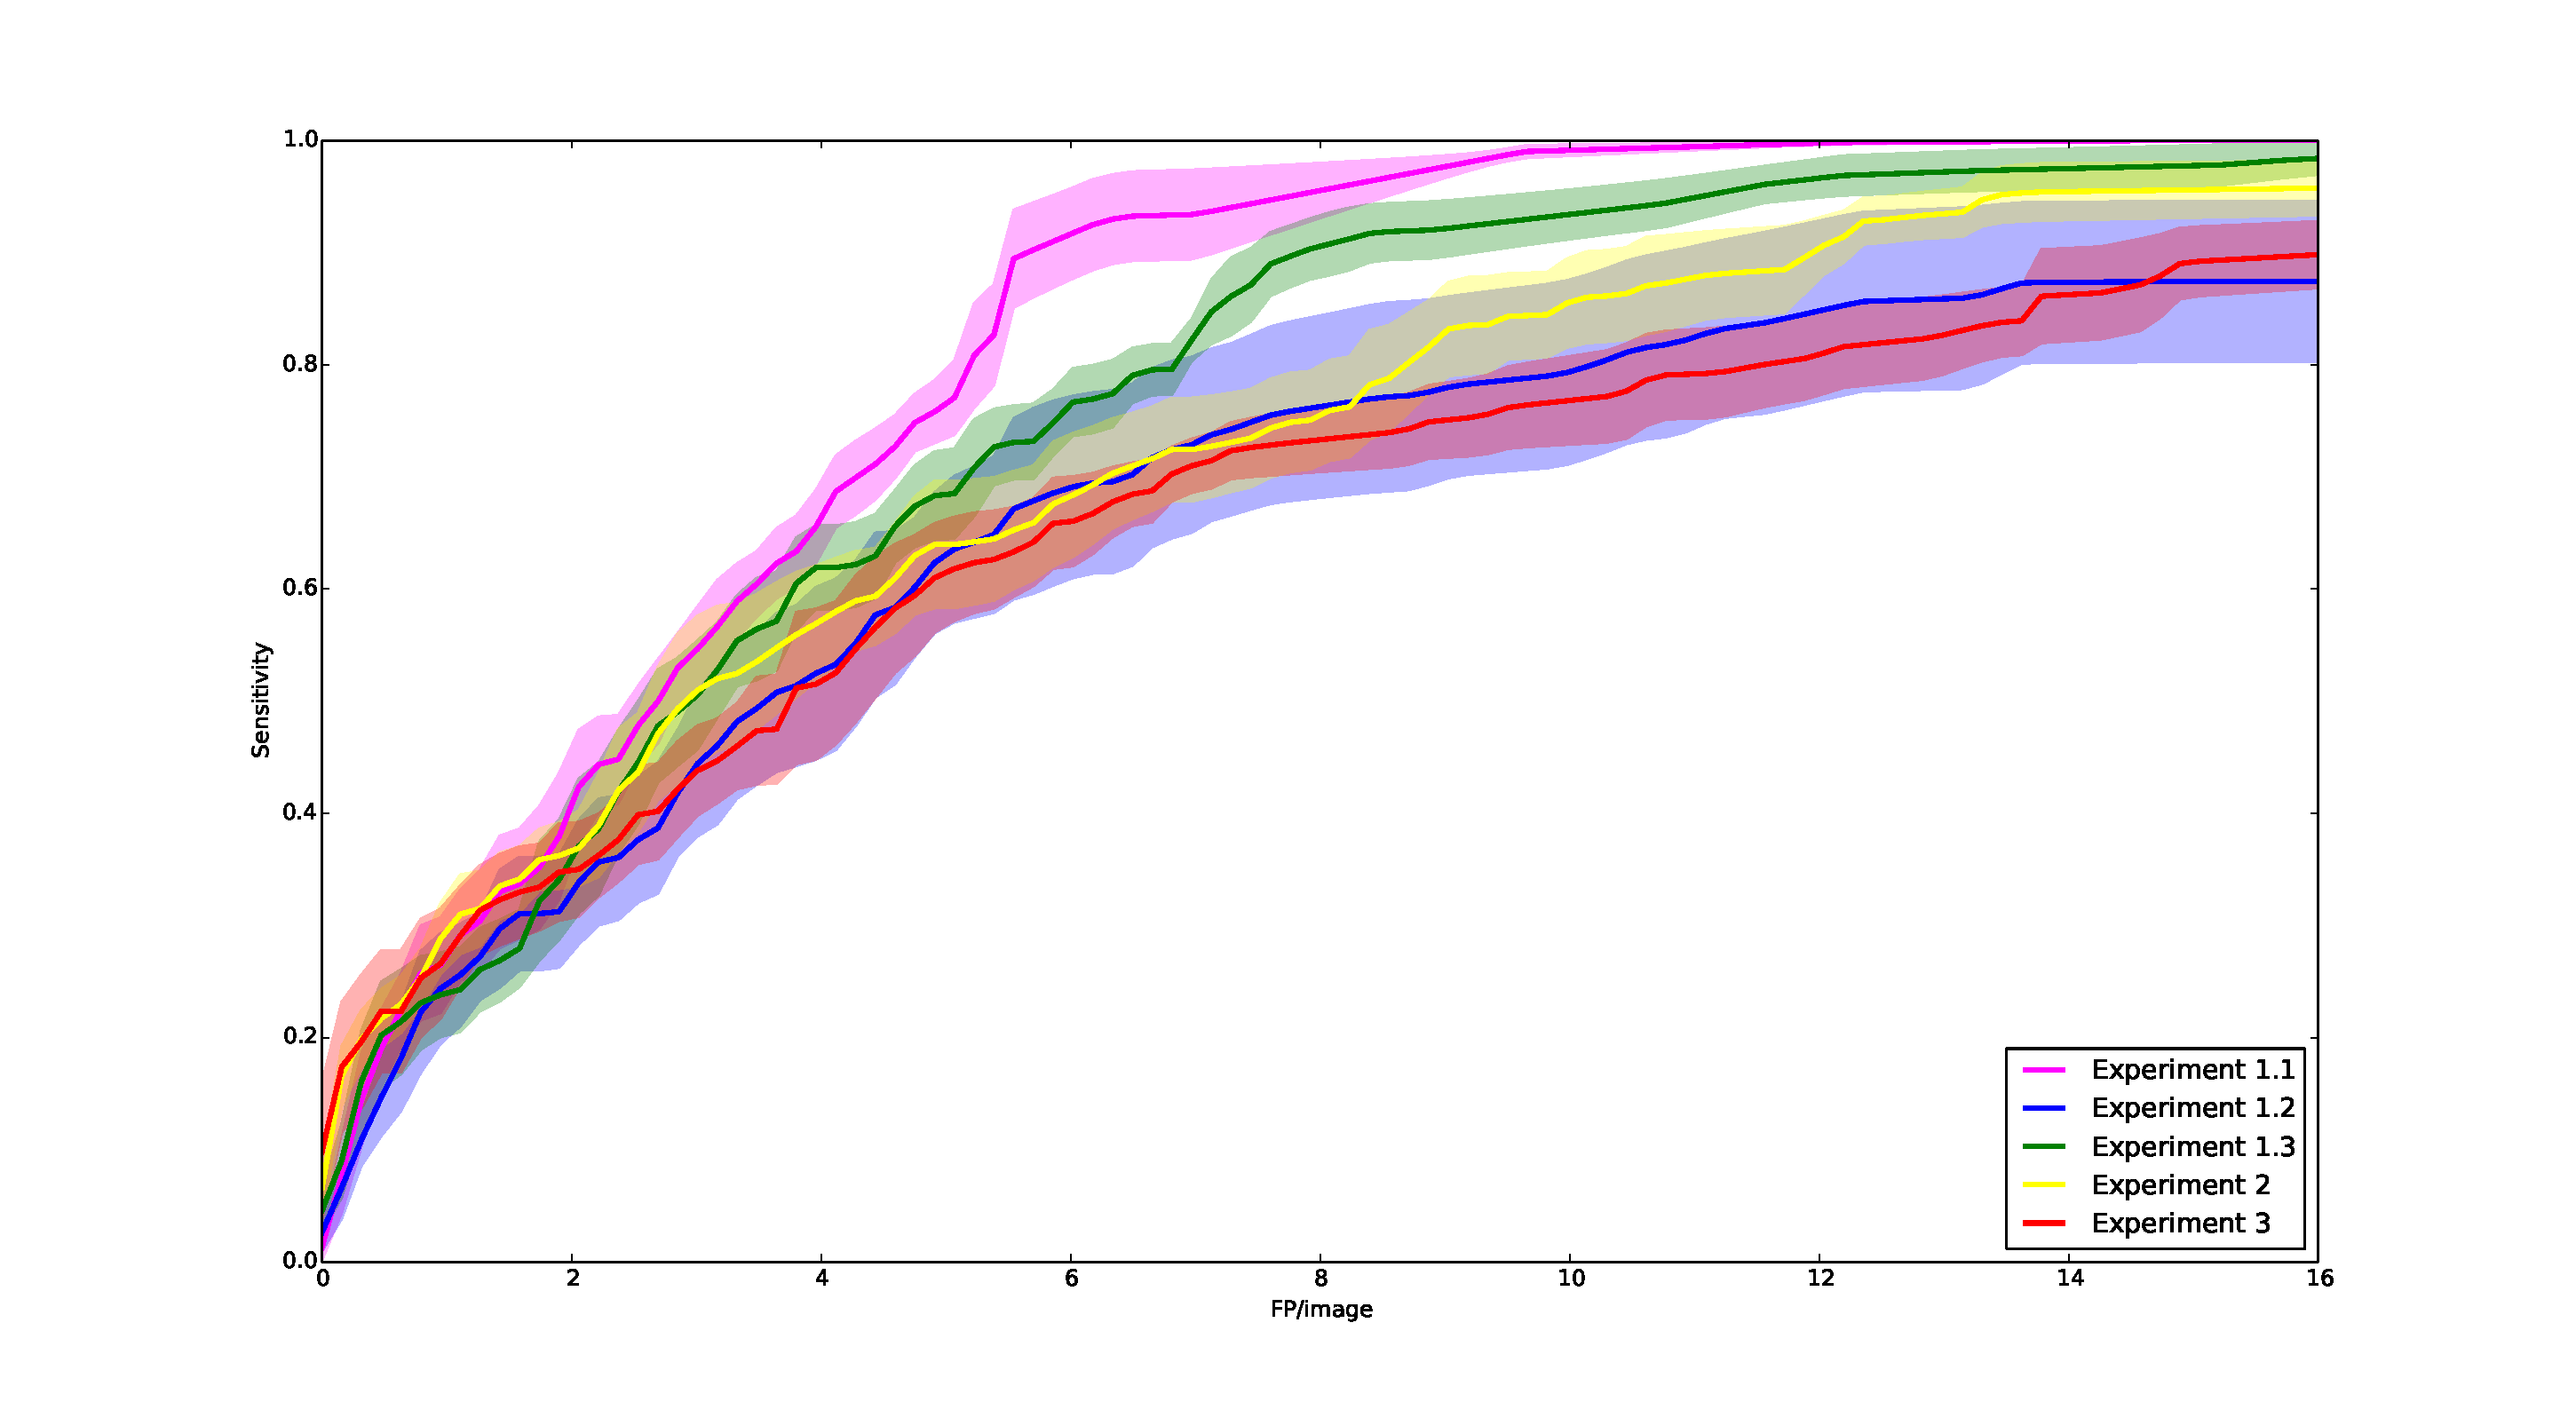
\includegraphics[width=\textwidth]{plots/FROC_plus_std.pdf}
	\caption[FROC curves]{Average FROC curves for every model. Shaded areas represent one standard error of the mean.}
	\label{fig:FROCResults}
\end{figure}

To better analyze our models we look at IOU as the probability threshold varies (Fig.~\ref{fig:IOUResults}): as expected, IOU starts at zero, increases gradually and decreases again as models go from predicting nothing as positive (low intersect) to predicting everything as positive (high union). Overall, curves for models 2 (yellow) and 3 (red) peak higher than those for other models, likely because they learn better feature representations. Model 1.1 (magenta), which is the only one that does not use a weighted function, performs better at lower thresholds because it only predicts low probabilities (less than 0.3); it is also the poorest performer, contrary to what the FROC curve may imply.
\begin{figure}[h]
	\centering
		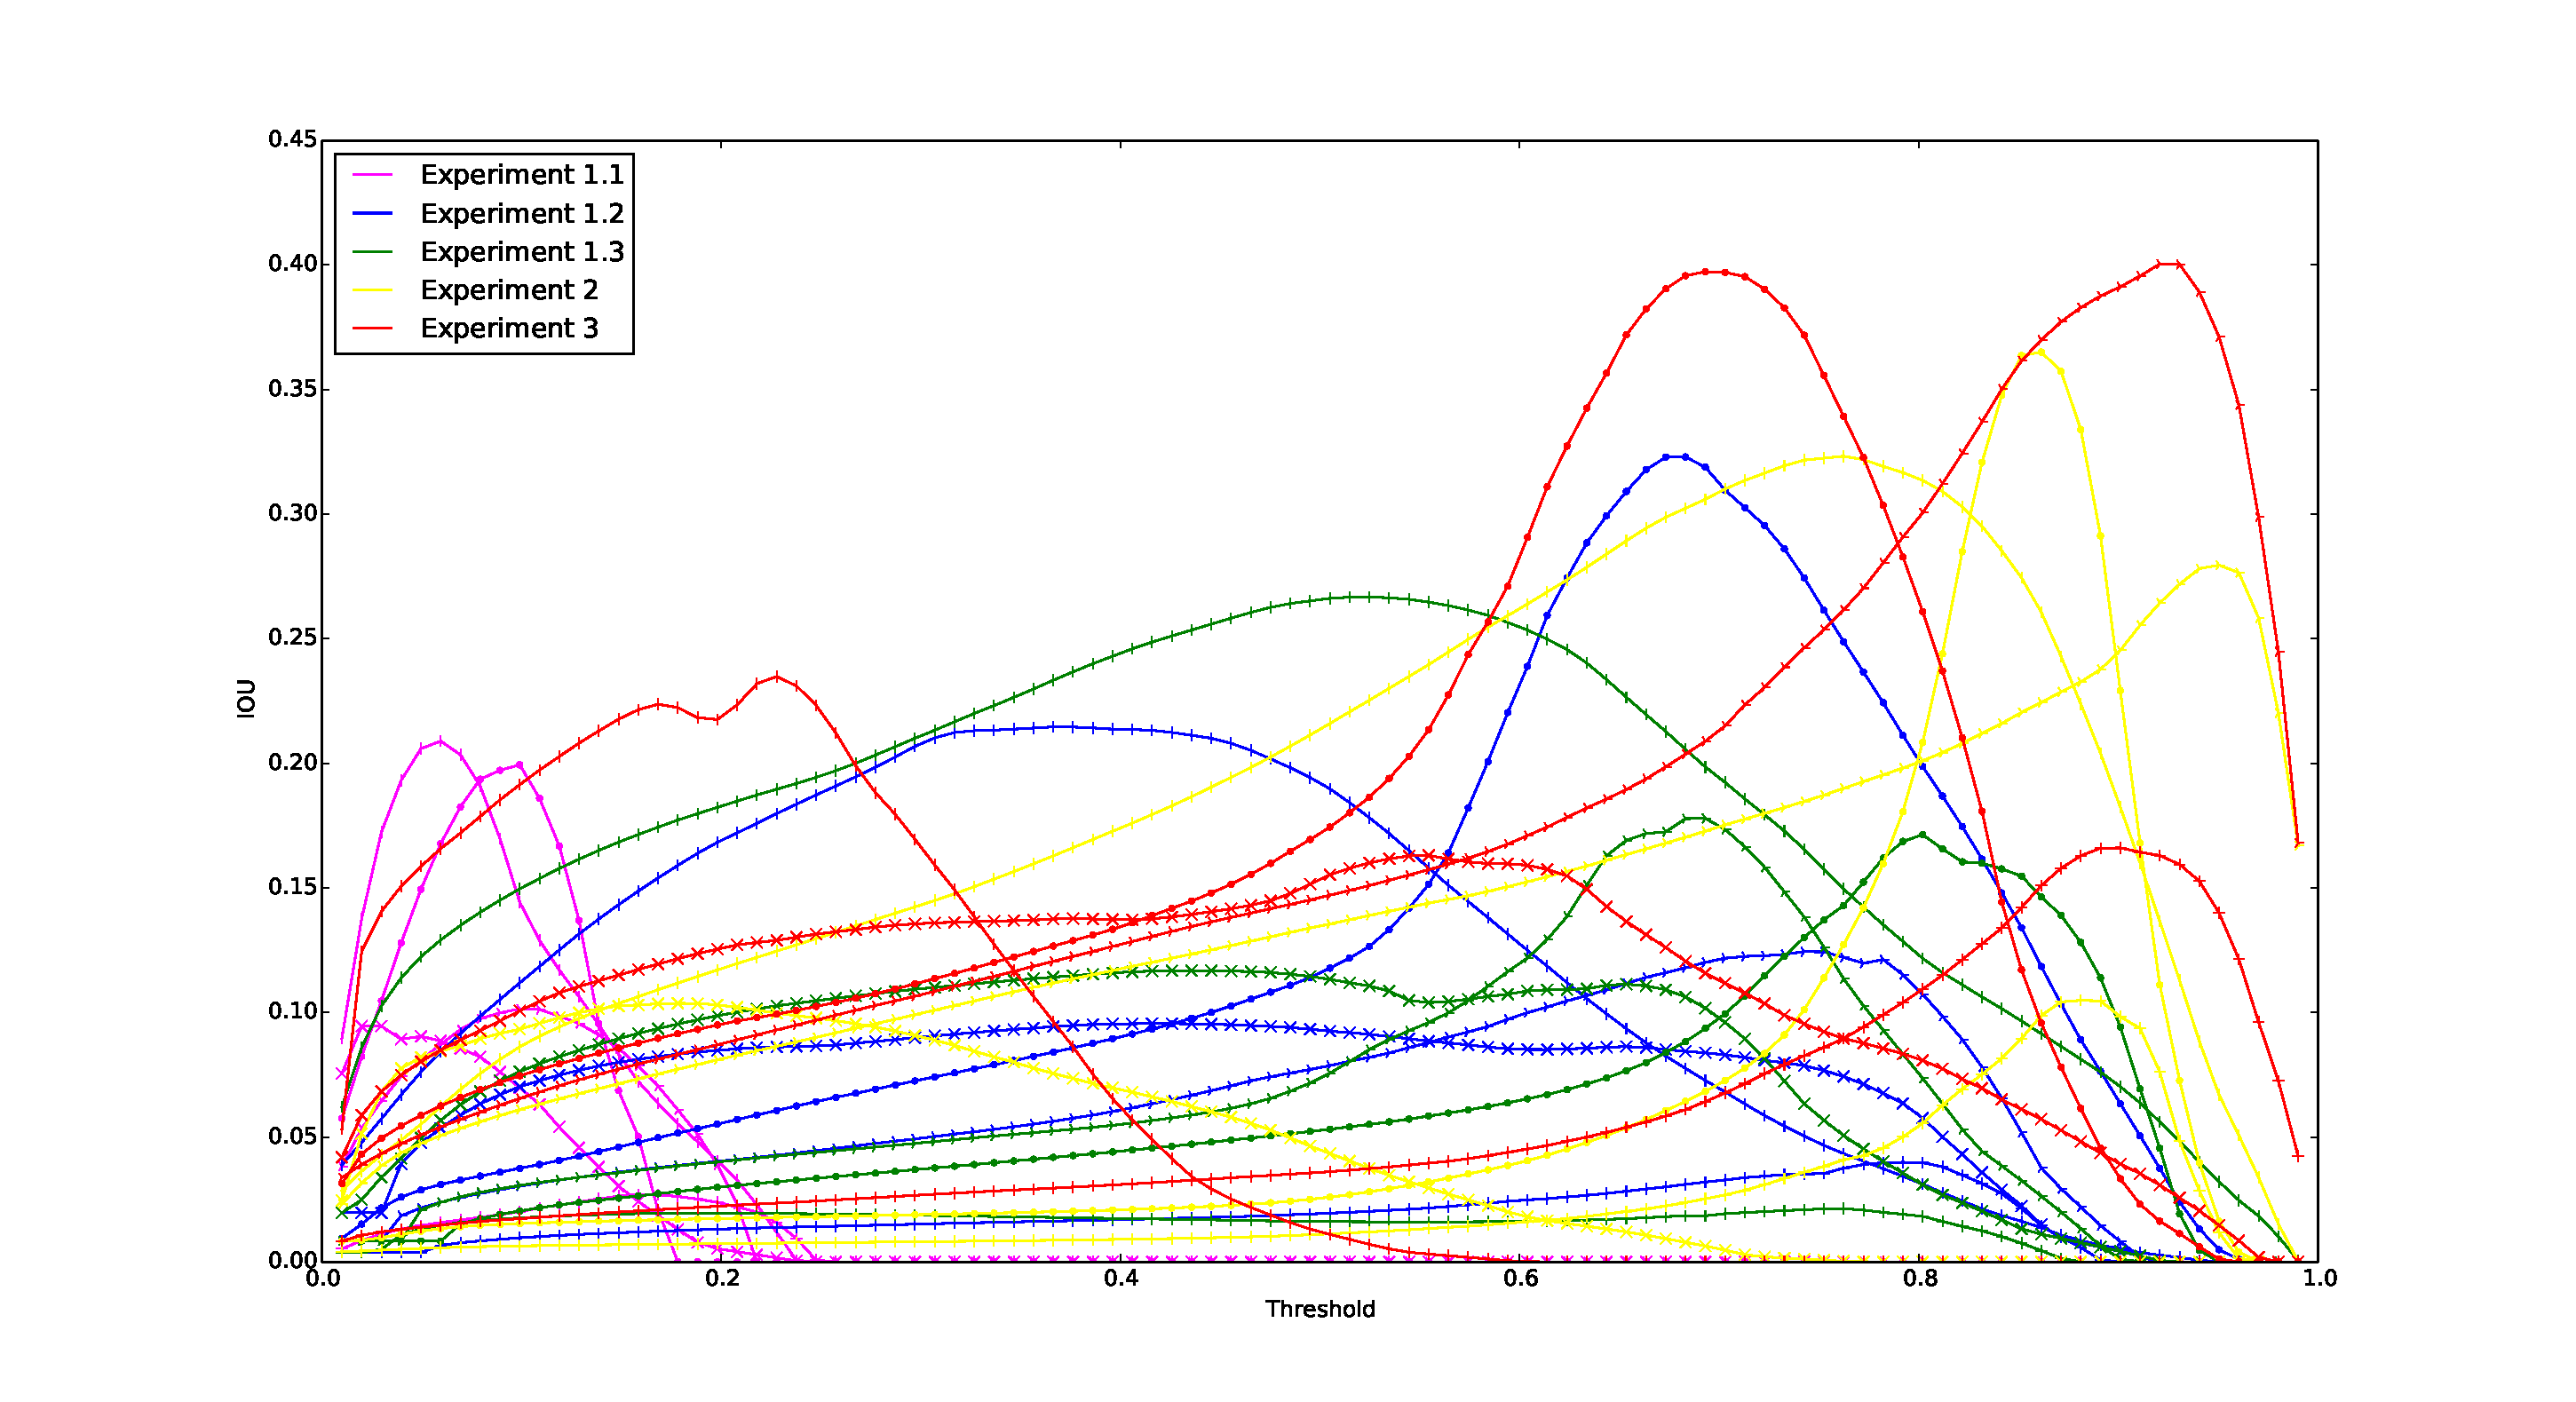
\includegraphics[width=\textwidth]{plots/IOU_all_folds.pdf}
	\caption[IOU curves]{IOU curves for every model and fold for varying probability thresholds. Experiments are drawn in different colors and markers are used to differentiate among folds.}
	\label{fig:IOUResults}
\end{figure}


%The highest peak in each curve represents the best possible IOU that a model could achieve.
%Peaks in each curve represent the best possible IOU that the model could achieve.
The highest peak in each curve represents the best possible IOU that a model achieves in that fold. Although this number is not valid on its own as, beforehand, we ignore what threshold produces it, it is a good proxy for performance and could be used to compare between models. We list these values in Table~\ref{tab:PeakIOUResults}. Once more, models 2 and 3 outperform the simpler architecture with model 3 producing the best results. Comparing experiments 1.1, 1.2 and 1.3, we notice that adding a weighted loss function improves performance while enhancing the images has little effect and may even be detrimental.
%The difference in average performance across folds (last row) shows that, even for the same model, some folds have better (or worse) results. 
The difference in average performance across folds (last row) shows that results also depend on the specific fold used. 
This variability would decrease if we used bigger test sets.
%This difference shrinks for bigger test sets.
\begin{table}[h]
	\centering
	\begin{tabular}{l*{6}{c}}
		\hline
		 & \textbf{Fold 1} & \textbf{Fold 2} & \textbf{Fold 3} &\textbf{Fold 4} &\textbf{Fold 5} & \textbf{Average $\pm$ SEM} \\
		\hline 
		Experiment 1.1	&0.03	&0.09	&0.21	&0.20	&0.10	&0.13 $\pm$ 0.03\\
		Experiment 1.2	&0.04	&0.10	&0.21	&0.32	&0.12	&0.16 $\pm$ 0.04\\
		Experiment 1.3	&0.02	&0.12	&0.27	&0.17	&0.18	&0.15 $\pm$ 0.04\\
		Experiment 2	&0.11 	&0.10	&\textbf{0.32}	&0.37	&0.28	&0.24 $\pm$ 0.05\\
		Experiment 3	&\textbf{0.17}	&\textbf{0.17}	&0.23	&\textbf{0.40}	&\textbf{0.40}	&0.27 $\pm$ 0.05\\
		Average			&0.07		&0.11	&0.25	&0.29	&0.22 &\\
		\hline
	\end{tabular}
	\caption[Peak IOU values for the final models]{Best possible IOU for each experiment. Best model in each column is shown in bold. SEM stands for standard error of the mean.}
	\label{tab:PeakIOUResults}
\end{table}

Lastly, we examine predictions made by our models to get a sense of their qualitative value (Appendix~\ref{app:examples}).
Models predict visually similar heatmaps but different models appear to produce better predictions for particular examples. Models 1.1, 1.3 and 3 are consistently good. On the downside, all models mark chest muscle with high probability and none is particularly good at localizing subtle lesions. It is also notable that model 1.1 is very conservative in its predictions while model 2 is quite more liberal, predicting large areas as probable masses.

\section{Discussion}
We found that convolutional networks are able to segment breast cancer masses as a single end-to-end model going from the original mammograms to a full-size prediction; this simplifies the complex pipeline of analysis used for current computer vision systems. We expect medical image analysis to benefit from adopting modern machine learning techniques to complement or replace more established systems. This work is a step in that direction and, to the best of the author knowledge, the first documented use of convolutional networks for breast cancer lesion segmentation.

Networks with many layers and number of parameters produced the best results regardless of the architectural details; however, our biggest model started to show signs of overfitting. Architectures with sufficient power learn the complex features needed for this task with ease. Finding a good learning rate proved neccesary for convergence while small changes in the regularization parameter did not affect learning.
% selecting a good learning rate proved necessary for convergence.  
Furthermore, using a weighted loss function stabilized training by allowing networks to focus on correctly classifying masses rather than normal breast tissue; it also encouraged networks to make predictions covering the entire probability range rather than being too conservative and predicting only low probabilities.
%Explain more here?
Models did not benefit from enhancing the input images. We believe complex networks benefit from details in the original image that enhancement vanishes. This is encouraging given our stated objective of blending all the processing pipeline into a single learnable step without reliance in expert knowledge of the application.

Convolutional networks, along other deep learning models, have been used succesfully in many computer vision and medical imaging tasks and some have started to be deployed in commercial and medical settings. Our results fall along these lines supporting convolutional networks as a promising technique for breast cancer systems.
% Our results

The main limitation of this work is the size of our data set that resulted in small test sets and high variability in performance estimates. For this reason we refrain from making strongs conclusions and focus on general trends that hold over all examples. Another possible criticism is that our models do not perform as well as more complex systems currently used for this task, although we can not make a direct comparison given the various metrics and forms of computation used. A bigger dat set could improve both of these shortcomings providing better estimates of performance and a richer training set. We have shown a succesful proof-of-principle but further research will be neded to confirm our insights and implement a functional system that could be deployed in real systems. % the way we test things is also weird.

%A couple of questions left unanswered are 
It is unclear whether convolutional networks will be able to take advantage of further examples or whether we will need to enrich our data by including other kind of lesions, acquisition configurations or density information. Based on their performance in other data-rich settings, we believe they are flexible enough to perform much better than achieved in this thesis and encourage work in this direction.

The significance of this work relies on the promise of machine learning boosting current CAD systems and the impact that even a small improvement could made in thousand of women. Achieving human or near-human performance in this tasks, as convolutional networks have been able to do in other computer vision tasks, could help radiologists and patients all over the world. We expect machine learning systems to play an important role in this quest.

\section{Summary}
All models produced good results with complex architectures performing better. Using a weighted loss function that gives more weight to errors committed on breast masses helped both with training and results while using a simple form of image enhancement did not. Results are promising but more research is needed before we can replace an entire mammographic systems with a single convolutional network.
